\documentclass[aspectratio=169,11pt]{beamer}
\makeatletter
\input{../../templates/dune-professional/beamerthemeDUNEProfessional.sty}
\makeatother
\title{Ground shakes}
\author{Manuel Arroyave}
\date{28 October 2026}
\renewcommand{\DuneDiagramCaption}[1]{{\small\color{DuneText}#1\par}}
\newcommand{\PlotNote}[1]{\smallskip{\footnotesize\color{DuneTextMuted}#1\par}}
\newcommand{\EDMS}[1]{\href{https://edms.cern.ch/document/3493627/1}{EDMS 3493627 v1, #1}}
\begin{document}

\begin{frame}{Ground shakes}
\framesubtitle{TPC, PDS and slow controls · ProtoDUNE-HD · Manuel Arroyave}
\begin{itemize}
\item We reviewed 1,531 records from seven runs.
\item The earlier slides already show the TPC precursor and electrical pickup in the PDS.
\item Here we look at the early PDS pulses, their timing and possible matches to charge.
\item We still need to establish which pulses are real light and where they come from.
\end{itemize}
\PlotNote{TPC: charge readout. PDS: light readout. Slow controls: voltage, current and other operating values.
Earlier observations: \EDMS{pp.\ 9, 21, 23, 79}.}
\end{frame}

\begin{frame}{Before the main shake}
\framesubtitle{Run 32731, event 33}
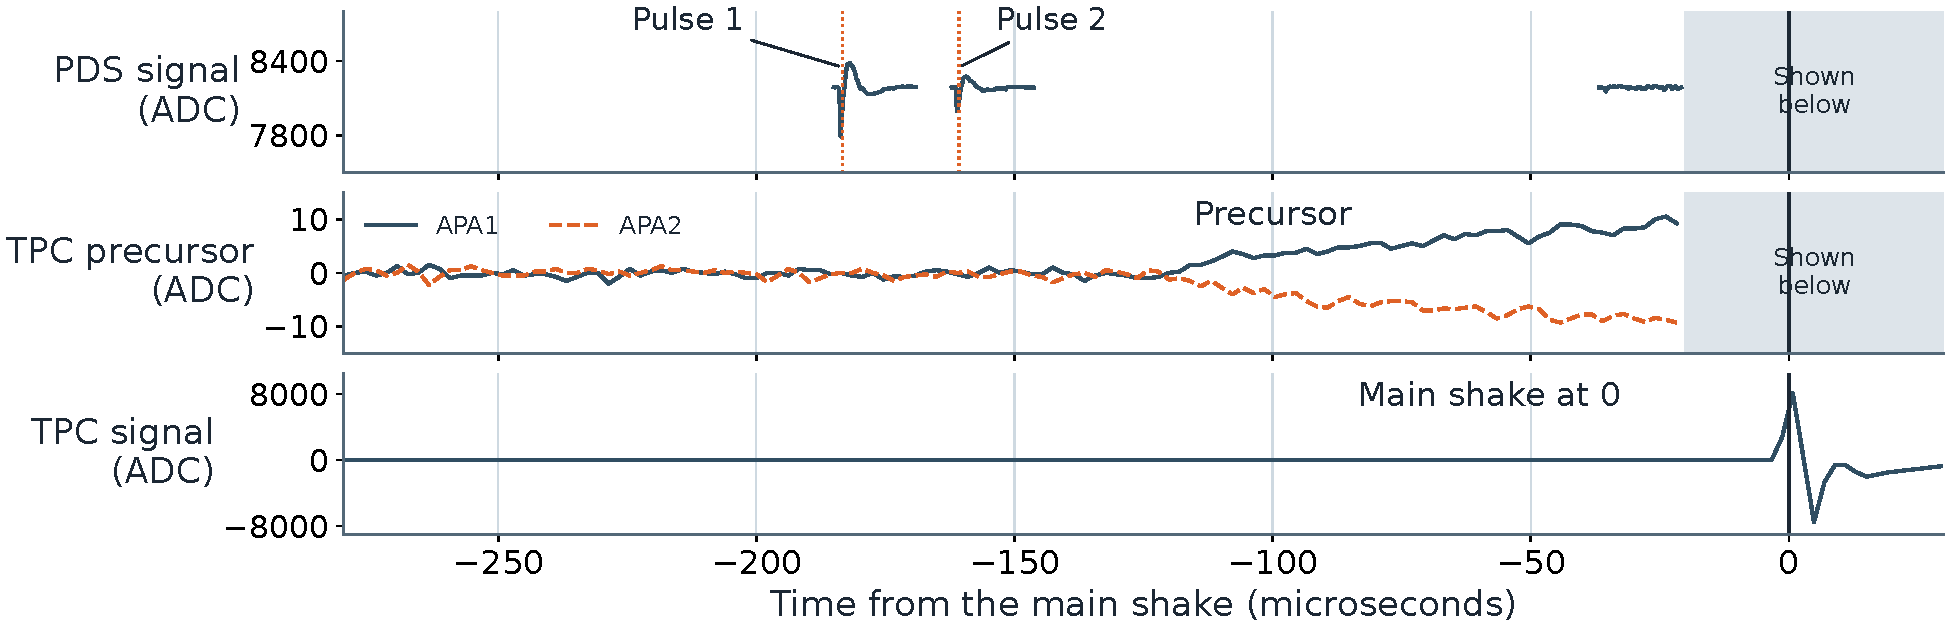
\includegraphics[width=\textwidth]{figures/10-event-sequence.pdf}
\DuneDiagramCaption{\textbf{Top:} two PDS pulses. \textbf{Middle:} the small TPC precursor.
\textbf{Bottom:} the main shake at time 0. In this event, the PDS pulses come before the small TPC rise.}
\PlotNote{The upper plots are magnified so we can see the small signals. Gaps mean missing or excluded samples.}
\end{frame}

\begin{frame}{Double pulses}
\framesubtitle{Two events from run 32731 · DAPHNE 109, channel 47}
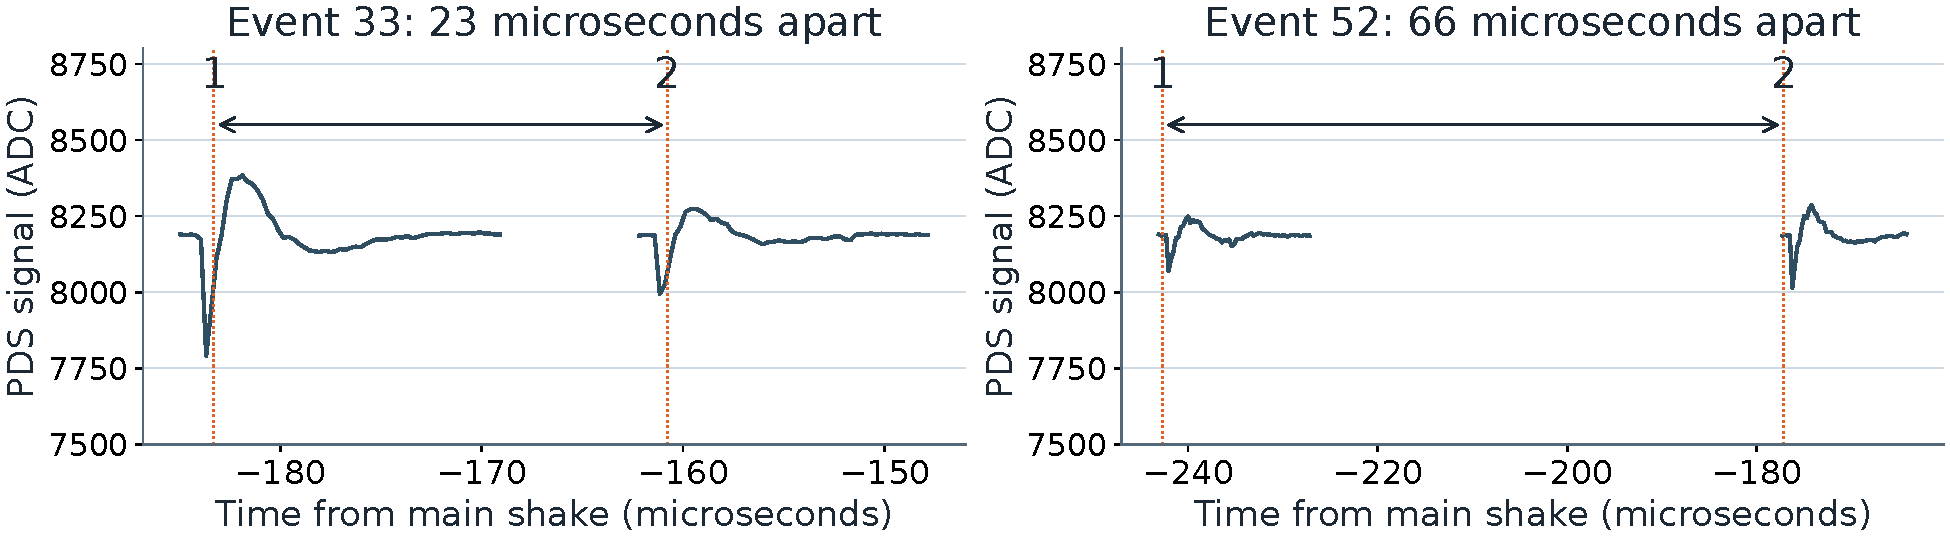
\includegraphics[width=\textwidth]{figures/11-double-pulses.pdf}
\DuneDiagramCaption{Each dip is a PDS pulse. The gaps are about 23 and 66 microseconds.
One source could produce pulses at different intervals.}
\PlotNote{We find two or more pulses in 101 of 716 events, searching 100--300 microseconds before the shake.
These are early pulses, before the main-shake reflections. We have not confirmed that they are light.}
\end{frame}

\begin{frame}{Timing of the early PDS pulse}
\framesubtitle{PDS time minus main-shake time · Negative means before the shake}
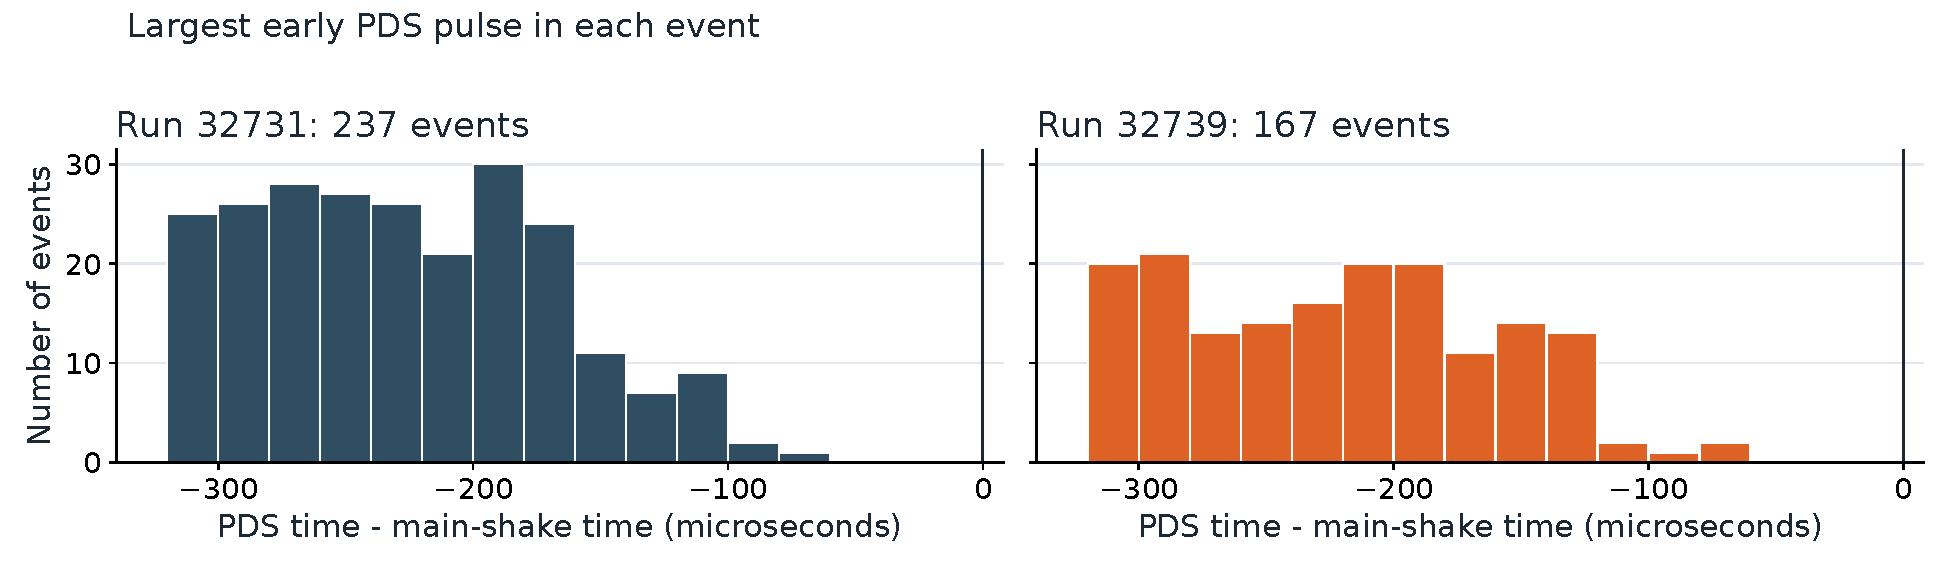
\includegraphics[width=\textwidth]{figures/15-pds-to-shake-histogram.pdf}
\DuneDiagramCaption{We take the largest sharp pulse before the TPC precursor in each event.
The times spread from 73 to 316 microseconds before the shake. The medians are 230 and 220 microseconds.}
\PlotNote{The pulse finder needs 21 channels. No event has that coverage earlier than about 320 microseconds before the shake.
The early tail is unmeasured, so we cannot tell whether the full distribution is Gaussian.}
\end{frame}

\begin{frame}{Time between TPC signals and PDS pulses}
\framesubtitle{The TPC signals are short groups of activity on neighbouring wires}
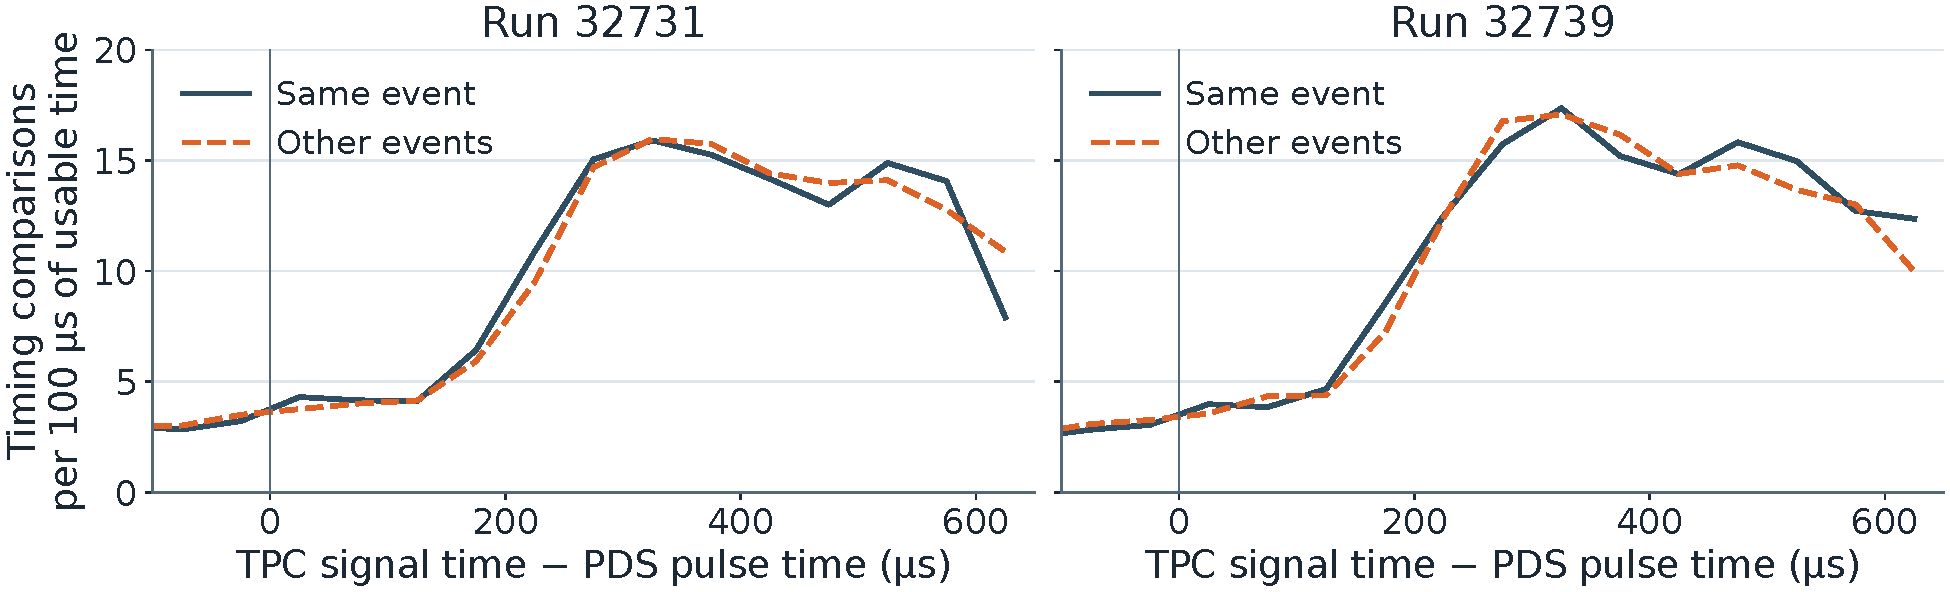
\includegraphics[width=\textwidth]{figures/05-charge-light-timing.pdf}
\DuneDiagramCaption{One entry is one selected TPC time minus one PDS pulse time.
We do not add or integrate the signals. \textbf{Blue:} times from the same event. \textbf{Orange:} PDS times from other events.}
\PlotNote{Y counts these comparisons per 100 microseconds of usable time. A comparison is not a confirmed physical match.
TPC signals can include electrical pickup. Repeated activity at one spot remains possible.}
\end{frame}

\begin{frame}{Next checks}
\begin{itemize}
\item Fit the charge tracks. Do different events point to the same place and the same light--charge delay?
\item For double pulses, look for two charge signals with the same gap and a common drift delay.
\item Recheck the PDS precursor as the wire bias changes in runs 30201 and 30202.
\item Compare with events without ground shakes, taken under similar conditions.
\end{itemize}
\PlotNote{The first three checks can use existing data. We still need a matched sample without shakes.
Earlier questions: \EDMS{pp.\ 34--35, 39, 42}.}
\end{frame}

\appendix
\begin{frame}{Backup: data and definitions}
\begin{columns}[T,onlytextwidth]
\begin{column}{0.40\textwidth}
\textbf{Saved 2024 records}\par\smallskip
{\small\renewcommand{\arraystretch}{1.16}
\begin{tabularx}{\linewidth}{@{}Xrr@{}}
\toprule Month & Run & Records\\\midrule
July & 27938 & 6\\ & 27951 & 19\\
October & 30201 & 44\\ & 30202 & 83\\
November & 32730 & 1\\ & 32731 & 716\\ & 32739 & 662\\
\midrule Total && 1,531\\\bottomrule
\end{tabularx}}
\end{column}
\begin{column}{0.56\textwidth}
\textbf{Charge readout (TPC)}\par
{\small Measures signals from drifting electrons. APA1 and APA2 are the two charge-readout assemblies used here.}\par\medskip
\textbf{Light readout (PDS)}\par
{\small Records photon-sensor signals and electrical interference. A PDS pulse is not automatically a light flash.}\par\medskip
\textbf{Slow controls (SC)}\par
{\small Operating monitors: 34 channels, 7.74 million archived samples.}\par
\end{column}
\end{columns}
\PlotNote{Automatic charge screen: 1,516 candidates, five below cut, ten unassessable.
Selected files do not measure shake rate. No candidate has a complete 4 ms of pre-shake PDS readout.}
\end{frame}

\begin{frame}{Backup: opposite signs in APA1 and APA2}
\framesubtitle{A larger sample of the pattern shown in \EDMS{pp.\ 14, 79}}
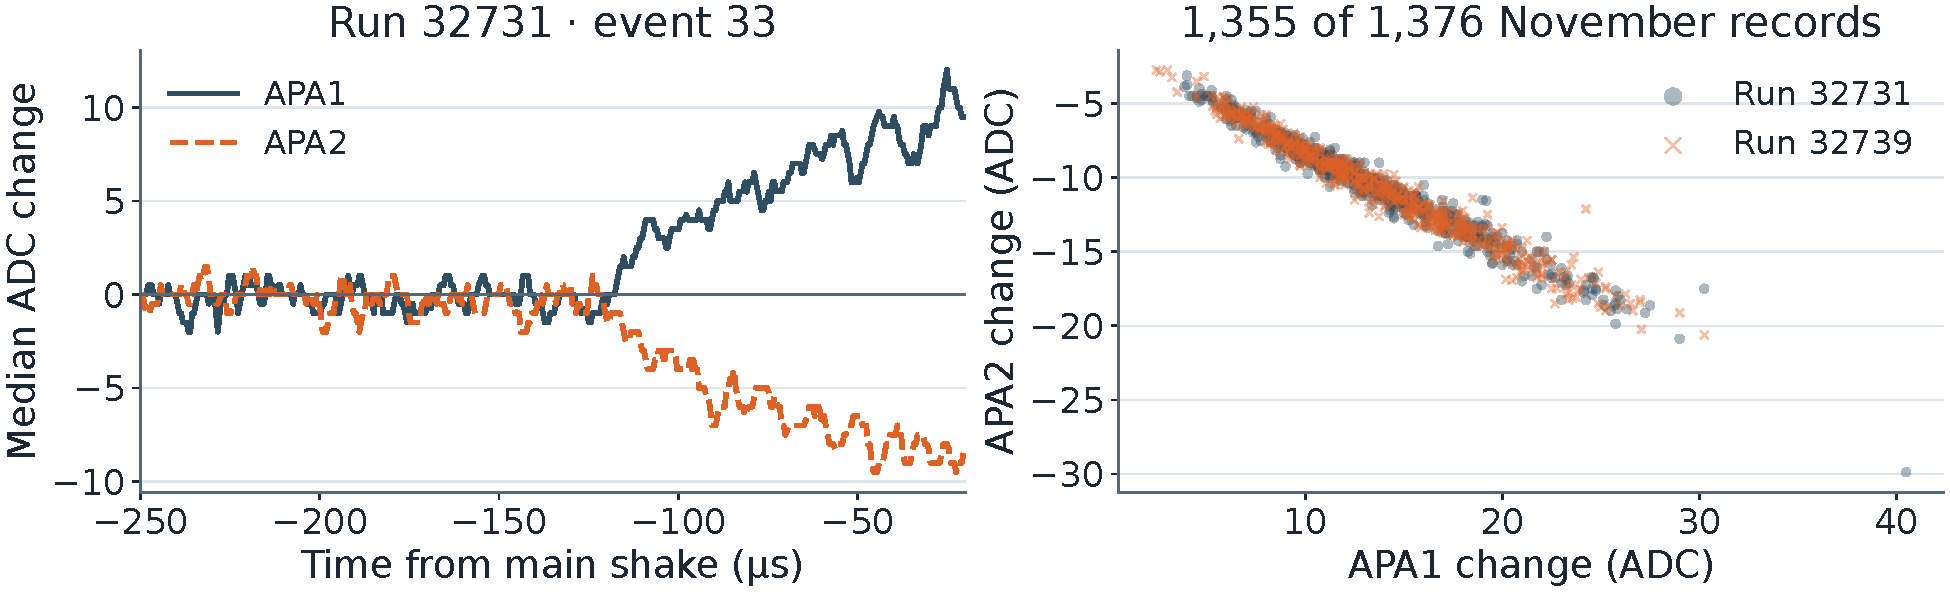
\includegraphics[width=\textwidth]{figures/02-opposite-charge-signs.pdf}
\DuneDiagramCaption{\textbf{Left:} APA1 rises while APA2 falls.
\textbf{Right:} one dot per event. We see both small precursors clearly in 1,355 of 1,376 November events.
The opposite signs were already known.}
\PlotNote{Median shape agreement after reversing APA2: 0.964 and 0.970.
These curves average the readout across each APA; they do not show individual charge tracks.}
\end{frame}

\begin{frame}{Backup: the fit depends on the channel}
\framesubtitle{The channel pattern was already shown in \EDMS{p.\ 21}}
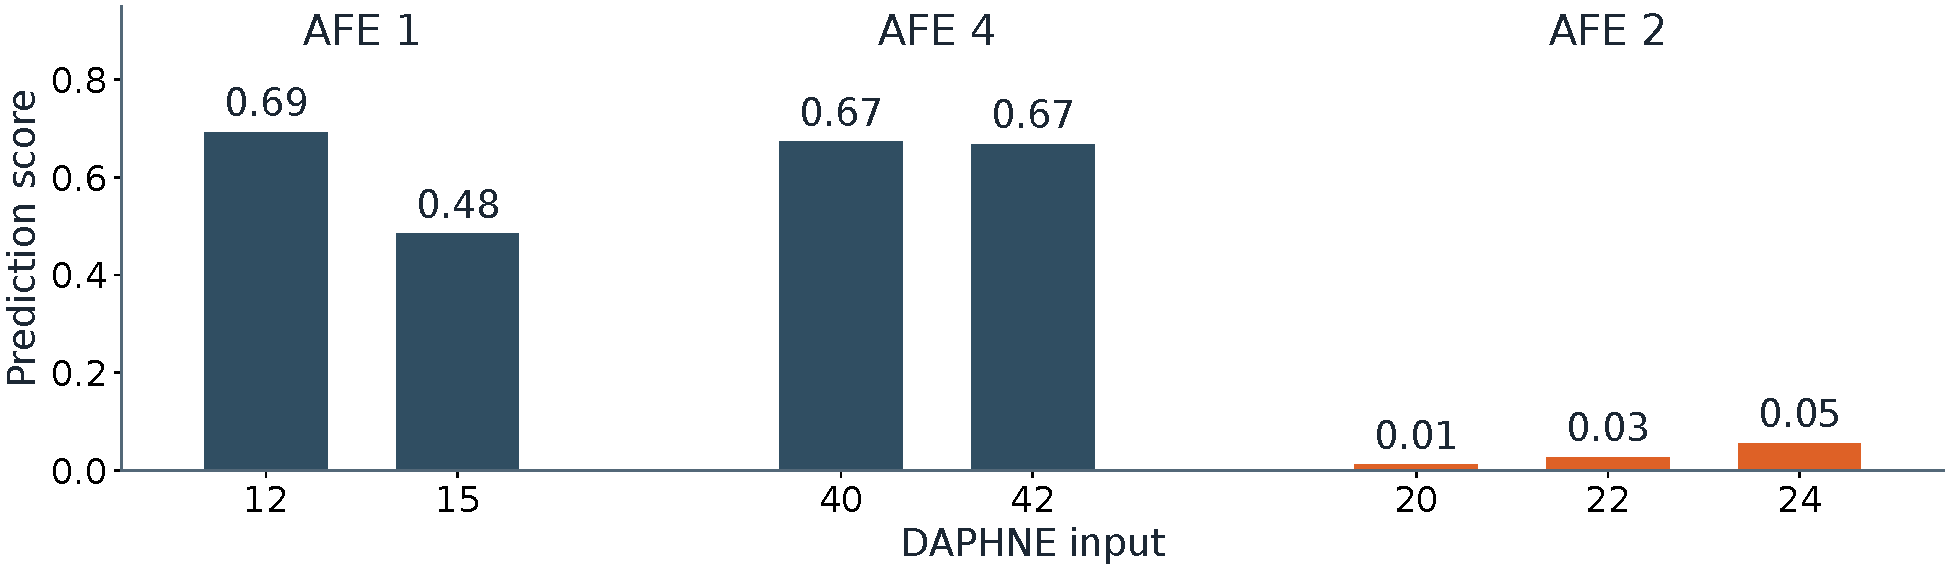
\includegraphics[width=\textwidth]{figures/08-electronics-groups.pdf}
\DuneDiagramCaption{Each bar is a connected channel. Taller bars mean that disconnected channels predict more of its signal.
The fit works much better for some groups than for others.}
\PlotNote{AFE: an eight-channel front-end chip. Score: 0 = no gain over a zero-change guess; 1 = exact prediction.
Trained on run 32731; tested on run 32739. A main-shake-trained fit fails on early pulses.}
\end{frame}

\end{document}
